\chapter{Tones: Theory and Computation} 
\label{chap:tones}

Languages with tonal distinctions have been studied as a more or less separate 
subfield known as tonal phonology. This division reflects a natural difference 
between the nature of tone and that of segments, as evidenced by a large body of 
empirical evidence from Asian and African languages. Rather than being inherent 
properties of vowels, tones may change independently of the segments that bear 
them. This property challenges traditional linear rule-writing approaches, which 
provide a cumbersome means of capturing tonal generalizations. Consequently, any 
discussion of tone necessarily involves a discussion of its representations, 
ranging from accent marks and feature-based representations to phonetically 
based notational systems \citep{chao1930system}. These approaches can be found 
throughout both the African and Asian tonal phonology literature. Among them, 
Goldsmith's (1976) autosegmental theory has become the most influential and widely 
adopted framework. The first half of this chapter provides an overview of the major 
approaches to tonal representation and typology.

The issue of representation further poses important requirements for computational 
modeling. Since the introduction of autosegmental theory by 
\citet{goldsmith1976autosegmental}, there has been a clear shift in theoretical 
phonology toward structurally enriched representations. In contrast, computational 
approaches have been slower to adopt such representations. 
Works by \citet{jardine16dissertation,chandlee2019autosegmental,oakden2020computational} 
argue that linguistically meaningful representations can reduce computational complexity. 
These representations include autosegmental graphs \citep{jardine16dissertation}, 
metrical structures \todo{lamount}, and feature-based representations for segmental 
learning \todo{magda}. These proposals, together with their computational 
implementations, highlight an important direction for computational modeling: 
the use of linguistically informed representations to improve interpretability, 
data efficiency, and linguistic adequacy through the development of small, 
specialized language models. The second half of this chapter reviews 
computational approaches to tonal phonology, including finite-state transducers 
and other computational models. It also discusses the challenges and 
opportunities involved in developing computational models that effectively 
capture the complexities of tonal phonology.

\section{Representations of Tone}

Estimates of the proportion of the world's tonal languages vary 
from 42.9\% \todo{thet}

\citet{yip2002tone}, for example, suggests that as many as 60--70\% of the world's 
languages may be tonal, whereas \citet{maddieson2013tone} estimates the proportion 
to be closer to 40\%. This discrepancy reflects differences in language sampling as 
well as in the criteria used to distinguish tone languages from languages with pitch 
accent or marginal tonal contrasts. Nevertheless, tone languages have a non-even 
geographical distribution: they are especially widespread in Africa, Central America, 
and East and Southeast Asia, while occurring more sparsely in Eurasia, North America, 
and Australia 
\citep{welmers1962, maddieson2013tone, kao2017phonological, 
	gordon2016phonological}.

Since tonal languages are widespread across different 
geographic regions, different conventions for representing 
tones have been developed to accommodate the languages in 
questions. \citet{yip2002tone} classified three main notational traditions 
for tones: Africanist, Asianist, and Central Americanist.
I group the latter two together for the present discussion since 
both use numerical notation, although they differ in how the numbers 
correspond to pitch levels and contours. 

It is worth mentioning that, in this section, I use the terms ``notation'' and 
``representation'' interchangeably. Although the two terms differ, all the methods 
discussed below have been used in theoretical or computational analyses of tonal 
phonology. I review five such systems: letter notation, number notation, feature-based 
representation, Q-Theory, and autosegmental representation. The first two function 
primarily as notational systems in previous work, whereas the remaining three are more 
formal representational frameworks that have also been applied beyond tonal phonology.

\subsection{Letter System}

An Africanist convention is to represent tone using accent marks. Tones are commonly 
marked with diacritics, even when they are not represented in a language’s everyday 
orthography. Table~\ref{tab:africanist} shows a basic system.
\begin{table}[ht]
	\centering
	\caption{Common Africanist tone notation}
	\label{tab:africanist}
	\begin{tabular}{lll}
		\hline
		\textbf{Tone} & \textbf{Symbol} & \textbf{Letter} \\
		\hline
		High      & \textit{á} & H      \\
		Low       & \textit{à} & L      \\
		Mid       & \textit{ā} & M      \\
		Falling   & \textit{â} & F   \\
		Rising    & \textit{ǎ} & R   \\
		%		Fall-rise & `\/\` & FR/HLH \\
		%		Rise-fall & \textit{a᷈} & RF/LHL \\
		\hline
	\end{tabular}
\end{table}

It should be noted that Africanist notation varies across linguists 
and languages. First, the unmarked tone in a two-tone system may be 
left without a diacritic; similarly, the mid tone is often unmarked 
in a three-tone system. Conversely, the macron (ā) is also used to 
indicate vowel length in some literature. 
\todo{Provide examples of unmarked-tone conventions in several African languages} 

Second, the notation of contour tones may be ambiguous, particularly 
in languages in which contour tones have greater distributional 
flexibility. As shown in Table~\ref{tab:africanist}, a falling tone 
may be written with a circumflex on the nucleus vowel (\textit{â}), 
on a long vowel (\textit{â:}), or on one element of a complex 
nucleus (\textit{âi}, \textit{ân}). Additionally, contour tones
can emerge in the surface form as a morphological or phonological processes, even though the language does not have underlying contour form. One practice is to distinguish underlying contour from deritational contour with F vs HL and R vs LH. but this praxrixe is 
not consistnetly used. therefore, contour tones may alternatively be represented as (\textit{áà} = \textit{â:}). In 
languages that permit both concave and convex contour tones, 
circumflex and caron diacritics alone may be insufficient to 
represent more complex contours unambiguously.\todo{Mende tonal 
notation system}

\begin{table}[ht]
	\centering
	\caption{Common Africanist tone notation}
	\label{tab:africanist_updated}
	\begin{tabular}{lll}
		\hline
		\textbf{Tone} & \textbf{Symbol} & \textbf{Letter} \\
		\hline
		High      & \textit{á} & H      \\
		Low       & \textit{à} & L      \\
		Mid       & \textit{ā} & M      \\
		Falling   & \textit{â,â:,áà} & F/HL   \\
		Rising    & \textit{ǎ} & R/LH   \\
		Fall-rise & `\/\` & FR/HLH \\
		Rise-fall & \textit{a} & RF/LHL \\
		\hline
	\end{tabular}
\end{table}

Although these rules describe the observed mappings, they obscure the generalization 
that the tonal components are preserved while the number of tone-bearing units is 
reduced. A representation that decomposes contour tones into sequences of level tones 
captures this generalization more directly.

\subsection{Phonetic-Based Notation}

In the Asianist tradition, tone is commonly represented using Chao’s five-level 
system \citep{chao1930system}. An example of this system is shown in Table~\ref{tab:cantonese-tones}, which lists the nine lexical tones of Cantonese.

\begin{table}[ht]
\centering
\caption{Lexical tones in Cantonese}
\label{tab:cantonese-tones}

\begin{tabular}{llll@{\qquad}llll}
\toprule
\multicolumn{4}{c}{Non-entering} &
\multicolumn{4}{c}{Entering} \\
\cmidrule(r){1-4}\cmidrule(l){5-8}
Tone & Value & Description & Example &
Tone & Value & Description & Example \\
\midrule
T1 & 55 & High level   & \textit{si1} `poem' &
T7 & 5  & High entering & \textit{sik7} `know' \\

T2 & 25 & High rising  & \textit{si2} `history' &
T8 & 3  & Mid entering  & \textit{sek8} `tin' \\

T3 & 33 & Mid level    & \textit{si3} `to try' &
T9 & 2  & Low entering  & \textit{sihk9} `eat' \\

T4 & 21 & Low falling  & \textit{si4} `time' &
   &    &               & \\
T5 & 23 & Low rising   & \textit{si5} `market' &
   &    &               & \\

T6 & 22 & Low level    & \textit{si6} `matter' &
   &    &               & \\
\bottomrule
\end{tabular}
\end{table}
 
Chao's system has been widely adopted in the study of Chinese languages and dialects.
The specific rules are as follows:
\begin{enumerate}[itemsep=1em, parsep=-1em]
	\item The natural pitch range of a speaker’s normal voice is divided into five levels, with 1 representing the lowest pitch and 5 the highest.
	\item A sequence of digits indicates the starting point, turning point(s), and the endpoint of a pitch contour. 
	\item A toneless or neutral-tone syllable may be represented by 0.
	\item An entering-tone syllable—that is, a syllable ending in a stop coda—is conventionally represented by a single digit.
\end{enumerate}

In Central Americanist notation, tones are represented in a similar way, but in a 
reversed order, with 1 representing the highest pitch and 5 the lowest. This system 
is used in the study of Mayan languages, such as K’iche’ and Q’eqchi’. 

This way of representing tones is effective in describing their productive
and perceptual details. However, this can also leads to its limitation
and explains why such system is more treated as a notation rather than a formal mental representation of speakers. Transcriptions of the same languages can vary greatly across
linguists due to allphonic (or allotonic) and interspeakers variability. 
Take Shanghai Chinese (also known as Shanghainese, a variaty in Wu Chinese) as an example. Shanghainese has five tones, and their tone values have had different numerical
descriptions from different sources, as shown in Table~\ref{tab:shanghai-tones}.

\begin{table}[ht]
\centering
\caption{Tone values reported across different sources}
\label{tab:shanghai-tones}
\begin{tabular}{lccccc}
\toprule
& \multicolumn{5}{c}{Tones} \\
\cmidrule(lr){2-6}
Sources & T1 & T2 & T3 & T4 & T5 \\
\midrule
JSS 1960          & 53              & 34               & 13 / 14           & 5                & 2               \\
Walton 1983       & 53              & 34               & 14                & 5                & 2               \\
Xu et al. 1981--83 & 53             & 34               & 13                & \underline{55}   & 12              \\
Xu \& Tang 1988   & 53 / \underline{52}
                  & 334 / \underline{434}
                  & 113 / \underline{223}
                  & \underline{55} / \underline{54}
                  & 12 / \underline{23} \\
T. Shen 1981 (1985)
                  & 52
                  & 334 / 34
                  & 113 / 13
                  & 4 / 5 / 7 (\underline{45})
                  & \underline{23} \\
Yuan 1983         & 42              & 34 / 434         & 24                & 5                & \underline{23}  \\
Norman 1988       & 42              & 35               & 24                & \underline{55}   & \underline{23}  \\
\bottomrule
\end{tabular}
\end{table}

Obviously, tonal processes can be generalized using this numerical system, but 
the generalization appears to involve arbitrary changes in pitch values (which is, 
as the reader progresses in Section \todo{later}, same issues for feature system). 
For example, the fall-rise tone (T3) in Mandarin is consistently transcribed as 214. 
When two fall-rise tones are adjacent, the former one will undergo a sandhi process
and become a high rise. This process is formalized as 214 + 214 = 35 + 214. 
Although, this gives a clear depiction of the phonetic details, but the relationship 
between 214 and 35 appears arbitrary and does not reveal the phonological structure 
underlying the change. 

\subsection{Tonal Feature}
From this section onward, we shift from tone ``notations'' to 
attempts of their mental ``representations''. In segmental 
phonology, consonants and vowels are represetned
as a matrices of feature values, where every segment has its
distinctive features to seperate itself from others.

\todo{SPE, Pike, Woo etc}

\citet{sy1967phonological} proposes one
of the earliest feature theories of lexical tones to compensate
for the numerical system does not directly reveal the
phonological structure of tones, and enable tones to be studied 
in natural classes and typology. Wang uses the feature \textsc{[$pm$contour]} to
distinguish level tones from contour tones; the three features
\textsc{[$pm$High]}, \textsc{[$pm$ Central]}, and \textsc{[$pm$Mid]} to represent
pitch height; \textsc{[rising]} and \textsc{[falling]} to describe the
direction of pitch movement; and \textsc{[convex]} to distinguish
rise--fall contours from fall--rise contours. These features are shown
in Table~\ref{tab:tone-feat-matrix}.

\begin{table}[ht]
\centering
\caption{Tones and their features}
\label{tab:tone-feat-matrix}
\setlength{\tabcolsep}{5pt}
\begin{tabular}{l*{13}{c}}
\toprule
Tone 
& 1
& 2
& 3
& 4
& 5
& 6
& 7
& 8
& 9
& 10
& 11
& 12
& 13
\\
Feature
  & \tone{55}
  & \tone{11}
  & \tone{44}
  & \tone{22}
  & \tone{33}
  & \tone{25}
  & \tone{14}
  & \tone{53}
  & \tone{31}
  & \tone{535}
  & \tone{313}
  & \tone{453}
  & \tone{131} \\
\midrule
Contour
  & $-$ & $-$ & $-$ & $-$ & $-$
  & $+$ & $+$ & $+$ & $+$ & $+$ & $+$ & $+$ & $+$ \\

High
  & $+$ & $-$ & $+$ & $-$ & $-$
  & $+$ & $-$ & $+$ & $-$ & $+$ & $-$ & $+$ & $-$ \\

Central
  & $-$ & $-$ & $+$ & $+$ & $+$
  & $-$ & $-$ & $-$ & $-$ & $-$ & $-$ & $-$ & $-$ \\

Mid
  & $-$ & $-$ & $-$ & $-$ & $+$
  & $-$ & $-$ & $-$ & $-$ & $-$ & $-$ & $-$ & $-$ \\

Rising
  & $-$ & $-$ & $-$ & $-$ & $-$
  & $+$ & $+$ & $-$ & $-$ & $+$ & $+$ & $+$ & $+$ \\

Falling
  & $-$ & $-$ & $-$ & $-$ & $-$
  & $-$ & $-$ & $+$ & $+$ & $+$ & $+$ & $+$ & $+$ \\

Convex
  & $-$ & $-$ & $-$ & $-$ & $-$
  & $-$ & $-$ & $-$ & $-$ & $-$ & $-$ & $+$ & $+$ \\
\bottomrule
\end{tabular}
\end{table}

Under this theory, H, L, R, F, the common tones in african languages,
can be presented as [+H,-contour], [-H,-contour], [-H,+contour], [+H,+contour]. In other words, R
and F will be a natural class of [+contour] and L and R will be [-H].
For Mandarin Chinese, only two features are able to distinguish the
froru tones, see table~\ref{tab:mandarin-tone-features} 

\begin{table}[ht]
    \centering
    \caption{Pekingese tones represented by features}
    \label{tab:mandarin-tone-features}
    \begin{tabular}{lcccc}
        \toprule
        & Tone 3 [214] & Tone 4 [51] & Tone 2 [35] & Tone 1 [55] \\
        \midrule
        \textsc{Falling} & $+$ & $+$ & $-$ & $-$ \\
        \textsc{Rising}  & $+$ & $-$ & $+$ & $-$ \\
        \bottomrule
    \end{tabular}
\end{table}

Mandarin third-tone sandhi can now be represented as follows. 
Compared with the numerical notation, this generalization 
reveals more clearly that a fall--rise tone loses its falling 
component when it precedes another fall--rise tone.

\ex
\text{[+falling]} $\rightarrow$ [-falling] /
\text{[\underline{\hspace{1em}}, +rising]}  [+falling, +rising]
\xe

One property of this feature system is that it treats contour tones as
single units. However, \todo{woo} argues that contour tones should 
be decomposed into sequences of level tones. Thus, whether contour 
tones should be represented as single units is an important question 
for feature theories of tone.

Example~\ref{ex:cantdo} presents two common processes: H becomes R 
after {L, F}, and L becomes F after {H, R}. These processes cannot be
described using the feature \textsc{[contour]} because neither {L, F}
nor {H, R} forms a natural class in this system. Moreover, the theory
predicts unattested patterns, as shown in Example~\ref{ex:unattested}.

\ex \label{ex:cantdo}
H $\rightarrow$ R / \{L,F\} \_\_\\
L $\rightarrow$ F / \{H,R\} \_\_
\xe 

\ex \label{ex:unattested}
*[+H] $\rightarrow$ [+contour] / [-H]\_\_  \hfill equivalent to H $\rightarrow$ F / \{L,R\} \_\_\hfill(unattested)\\
*[-H] $\rightarrow$ [+contour] / [+H]\_\_\hfill   equivalent to L $\rightarrow$ R / \{H,F\} \_\_ \hfill(unattested)
\xe

There are also other attempts to adopt features to tone fields.
\cite{zhu1999shanghai} merged Chao's phonetic notation and feature
system, with one added feature - [Register] to captures the register
issues in many chinese dialects. Schachter and Fromkin’s (1968) landmark
generative phonology of Akan (Kwa, Ghana) describes a high tone
unassociated with a tone­ bearing unit (TBU) as [+seg, +tone, ØF]. 

\subsection{Q-Theory}

\citet{inkelas2013abc+} introduced \textit{Q-theory}, initially designed to account
for complex diphthongs and later expanded to contour tones. Under this
framework, each tone (or segment) can be divided into three temporally ordered,
quantized subsegments. A phonological representation follows the format
Q($q_1$, $q_2$, $q_3$), where a traditional representation, or a segment, can be
decomposed into three subsegments $q$. Here, ``q'' is loosely based on the concept
of quantized temporal subphases of the unit phonologists call a ``segment.''
A vowel with a rising-falling tone can be represented as
V(à\textsuperscript{1}á\textsuperscript{2}à\textsuperscript{3}).
\citet{inkelas2013abc+} argue that Q-theory can compensate for the difficulty of
Aperture Theory, which limits the number of aperture positions to a maximum of
two.

Q-theory is motivated by the typological observation that most complex tones do
not exceed three tonal levels and that four-tone contours are very rare
\citep{shih2013subsegmental}. It provides a useful harmony--disharmony typology
based on whether the target of change is the whole segment or a subsegment.

% See Table~\ref{tab:tone-harmony}.


% \begin{table}[htbp]
% 	\centering
% 	\caption{Tone harmony and disharmony involving whole segments and subsegments}
% 	\label{tab:tone-harmony}
% 	\begin{tabular}{lll}
% 		\hline
% 		& \textbf{Whole segment: Q} & \textbf{Subsegment: q} \\
% 		\hline
		
% 		\textbf{Harmony}
% 		&
% 		\begin{tabular}[t]{@{}l@{}}
% 			\textbf{a. Changzhi} \\
% 			(Duanmu 1994; a.o.) \\
% 			/kuə213-təʔ535/ $\rightarrow$ [kuə213-təʔ213] \\
% 			`pan, dim.'
% 		\end{tabular}
% 		&
% 		\begin{tabular}[t]{@{}l@{}}
% 			\textbf{c. Yoruba} \\
% 			(Akinbiyi \& Liberman 2001) \\
% 			/rárà/ $\rightarrow$ [rárâ] \\
% 			`elegy'
% 		\end{tabular}
% 		\\[2ex]
		
% 		\textbf{Disharmony}
% 		&
% 		\begin{tabular}[t]{@{}l@{}}
% 			\textbf{b. Pingyao} \\
% 			(Chen 1992; Yip 2002) \\
% 			/hai35 bing35/ $\rightarrow$ [hai53 bing35] \\
% 			`become ill'
% 		\end{tabular}
% 		&
% 		\begin{tabular}[t]{@{}l@{}}
% 			\textbf{d. Tianjin} \\
% 			(Chen 1985; a.o.) \\
% 			/feiL-jiL/ $\rightarrow$ [feiLH.jiL] \\
% 			`airplane'
% 		\end{tabular}
% 		\\
		
% 		\hline
% 	\end{tabular}
% \end{table}

The first limitation of Q-theory is that, even though the typological observation
suggests a lack of four-tone contours, there is in fact a typological category
found in some Chinese dialects known as the ``double circumflex''
\citep{zhu2012dipping}. Double-circumflex tones have two perceptually salient turning
points. Three variants of the double-circumflex tone can be distinguished by the
relative heights of these turning points, as shown in
Table~\ref{tab:double-circumflex}.

\begin{table}[htbp]
	\centering
	\caption{Three variants of double-circumflex tones}
	\label{tab:double-circumflex}
	\begin{tabular}{llll}
		\hline
		\textbf{Type} & \textbf{Contour} & \textbf{Variety} & \textbf{Example} \\
		\hline
		Back-low     & 4232 & Yuejiashan Mandarin (Zhongyang)
		& \textit{xiang} `make a sound' \\
		Equal-height & 3232 & Deqing Wu (Zhejiang)
		& \textit{ma} `hemp' \\
		Front-low    & 3242 & Qiyang Xiang (Hunan)
		& \textit{dong} `freeze' \\
		\hline
	\end{tabular}
\end{table}

One possible solution for accommodating these tones within Q-theory is to
consider a single contour (a fall or rise) as the subsegmental unit.
However, if a language with double-circumflex tones also has level tones (such
as 55) or short tones (also known as ``entered tone'', typically noted as 5), Q-theory is again insufficient to account
for all these tone types within a unified representation.

Secondly, Q-theory could also be seen as a flat-string version of a nonlinear
representation. Q could be seen as a tonal node, while its subsegments could be
seen as tone units. Whether a subsegment or the whole segment undergoes a change
also corresponds to the two tonal models proposed by \citet{yip1980chinese}
 and
\citet{bao1999structure}. \citet{jardine2021qtheory} argues that Q-theory is
logically equivalent to ARs under model theory and logical interpretations. This
means that, using a set of logical formulas, there is a bijective transduction
from one representation to the other, and vice versa. The differences are
presentational, but the representations are notationally equivalent.
\citet{oakdenNotationalEquivalenceTonal2020} provides a more detailed discussion
of notational equivalence.

\section{Autosegmental Theory}

Autosegmental theory marks a shift away from linear representations
of generative phonology developed in \textit{The Sound Pattern of English}
\citep{chomsky1968spe}. \citet{goldsmith1976autosegmental} proposes a
non-linear theory in which tones and segments are represented on separate
autosegmental tiers. 
\begin{quote}
In
autosegmental representation, however, we posit two or more parallel
tiers of phonological segments. Each tier itself consists of a string of
segments, but the segments on each tier differ with regard to what
features are specified in them.	
\citep[p.8]{goldsmith1976autosegmental}
\end{quote}

Elements on different tiers are linked by association lines, which are 
subject to a variety of well-formedness conditions and conventions. 
This framework provides the important insight that speech is
organized into parallel tiers and allows phonological representations to be
visualized as graph-like, multitiered structures. 
\begin{figure}[ht]
\centering
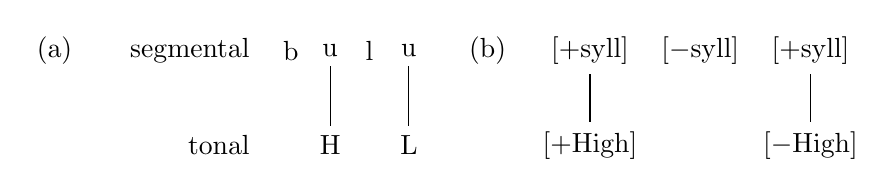
\begin{tikzpicture}[
    node distance=0.8cm,
    every node/.style={font=\normalsize}
]

% (a)
\node at (-1,1.2) {(a)};
\node[anchor=east] at (1.6,1.2) {segmental};
\node at (2.0,1.2) {b};
\node (u1) at (2.5,1.2) {u};
\node at (3.0,1.2) {l};
\node (u2) at (3.5,1.2) {u};

\node[anchor=east] at (1.6,0) {tonal};
\node (H) at (2.5,0) {H};
\node (L) at (3.5,0) {L};

\draw (u1.south) -- (H.north);
\draw (u2.south) -- (L.north);

% (b)
\node at (4.5,1.2) {(b)};
\node (syl1) at (5.8,1.2) {$[+\mathrm{syll}]$};
\node at (7.2,1.2) {$[-\mathrm{syll}]$};
\node (syl2) at (8.6,1.2) {$[+\mathrm{syll}]$};

\node (high) at (5.8,0) {$[+\mathrm{High}]$};
\node (low)  at (8.6,0) {$[-\mathrm{High}]$};

\draw (syl1.south) -- (high.north);
\draw (syl2.south) -- (low.north);

\end{tikzpicture}
\caption{Two representations of the same tonal structure.}
\label{fig:autosegmental-representations}
\end{figure}

A core mechanism and major advantage of autosegmental theory is that
associations can be manipulated independently of the elements they connect.
A phonological process may add or delete an association line without deleting
or changing the associated tone or segment. This separation makes it possible
to represent phenomena such as tone spreading, delinking, floating tones,
and contour tones in a unified way.


\citet{goldsmith1976autosegmental} formalizes a set of well-formedness
conditions (WFCs) governing the relationship between tones and the units
that bear them and require association changes to be minimal while 
maximising satisfaction of basic representational requirements.
In their original formulation, these conditions require
every vowel to be associated with at least one tone, every tone to be
associated with at least one vowel, and association lines not to cross.
\begin{enumerate}
    \setlength{\itemsep}{0em}
    \setlength{\parskip}{0em}
    \item All vowels are associated with at least one tone.
    \item All tones are associated with at least one vowel.
    \item Association lines do not cross (the No-Crossing Constraint, NCC).
\end{enumerate}

The significance of autosegmental theory extends beyond its ability to
provide simple formalizations of tonal association. As
\citet{leben2018history} comments, ``these simple rules interacted in
different ways in different languages, expressing patterns that might be
language-particular but using mechanisms that were universal''

The rest of this section demonstrate how autosegmental representations
capture tonal processes in both African and Asian languages more effectively
than string-based representations. These processes also serve as case studies
in later chapters.



\subsection{Tone Autonomy}
A central claim of autosegmental theory is that tones can behave
autonomously from the segments that bear them. This autonomy is not
directly captured by linear representations, in which tones and segments
are encoded as one unit. One evidence that challenge this practice comes
from vowel deletion: deleting a vowel does not necessarily delete its
associated tone. Instead, the tone may survive and reassociate with a
neighboring tone-bearing unit. Such patterns provide evidence that tones
and segments must be represented as distinct phonological objects.

This subsection examines vowel-deletion processes in three languages:
Engenni, Etsako, and Ogoja Yala \citep{kao2017phonological}. In all three
languages, the first vowel in a hiatus sequence is deleted.
However, the tone originally associated with V1 undergoes a 
different process in each language. I classify these
patterns as (1) host-dependent deletion, (2)
{position-based preservation}, and (3) {quality-based 
preservation}. From an autosegmental perspective, the three patterns show that how a change
on the segmental tier may trigger different adjustments on the tonal tier.

Let us first examine an example from Engenni compounds - this is a 
pattern where I refer as host-dominant. When vowel
hiatus arises at a morpheme boundary, the first vowel in the sequence
V1 is deleted, while the second vowel V2 survives. What,
happens to the tone borne by the deleted vowel? The answer is
simple: it is deleted along with its host.

\ex 
\textbf{Engenni (tone deletion):} 
Deleting the vowel also removes its associated tone.
\begin{multicols}{2}
\quad\ L\quad H\qquad\qquad H\\
 /\` ɔkò \# édèì/ $\rightarrow$ [\` ɔkédèì] \\
 \textit{man \ \ canoe} $\rightarrow$ \textit{``a man’s canoe"} 
 
 \quad\ \ H\quad L\qquad\qquad\ \ \ L\\
/fùnú \# èdhí/ $\rightarrow$ [fùnèdhí] \\
\textit{climb \ \ palm tree} $\rightarrow$ \textit{``to climb a palm tree"}
\end{multicols}
\xe


The second pattern is found in Etsako, a tonal Niger-Congo language
\citep{elimelech1976}. Unlike in Engenni, the tone T1 originally
associated with V1 is not deleted with its segmental host.
Instead, T1 survives and reassociates with its cloest available host V2. 
Consequently, $V_2$ bears both $T_1$ and its original tone, $T_2$. 
The two tones preserve their original order and combine to form a contour 
tone. I refer to this pattern as \textit{position-based preservation}, 
because the outcome preserves both tones and their order rather than 
selecting a tone on the basis of its tonal value.

\ex \textbf{Estako (contour formation):} 

\begin{multicols}{2}
\quad\ \ L \ \ \ H\qquad\qquad LH\\
/ówà \# ówà/ \ $\rightarrow$ [ówǒwà] \\
\textit{house \ \ house} $\rightarrow$ \textit{``every house"}

\qquad\ H \ \ \ L\qquad\qquad HL\\
/\`ɔ \# dé \ \# àkpà/ $\rightarrow$ [\`ɔdâkpà] \\
\textit{he \ \ buy \ \ cup}\quad$\rightarrow$ \textit{``he buys a cup"}
\end{multicols}
\xe

The third pattern is found in Ogoja Yala. Here, the outcome is determined
by competition between pitch values: the tone with the higher pitch always
survives, regardless of whether the winning tone was originally associated
with the deleted vowel or the surviving vowel. A high tone is preserved
whenever one is present, whereas a low tone is deleted whenever it competes
with a higher tone. If the two tones have the same value, it does not matter
which one survives, since there is no difference in the surface form. What could change is M tone, which could be deleted if it's next to a H or presrve if it is L. This
pattern can therefore be described by the tonal hierarchy H > M > L. I
refer to it as \textit{quality-based preservation} because the surviving
tone is selected according to its tonal value rather than its original
position.


\ex \textbf{Ogoja Yala (higher-pitch preservation)}
\begin{multicols}{3}
\quad L \; \  H \qquad \quad \ H\\
/dè \# áchí/ $\rightarrow$ [dáchí]\\
\textit{give \ grass} $\rightarrow$ \textit{``to give grass"}

\quad H\quad L\qquad\ \ \ \quad H\\
/má \# \` ɔchí/ $\rightarrow$ [m\' ɔchí]\\
\vspace{1em}\textit{see \quad tree} $\rightarrow$ \textit{``to see tree"}

\ \ M \ \ L \qquad \quad \ M\\
/b\=i \# \` ɔchí/ $\rightarrow$ [b\=ɔchí]\\
\textit{carry  stick} $\rightarrow$ \textit{``to carry a stick"}
\end{multicols}
\xe

\todo{add another example where vowel is quality senstive, but tone is not}

\subsection{Tone spreading and shift}
\citet{hyman2011tone} points a few aspects where tonal phonology distingusih itself
from segmental phonology. One striking property of tones is its long-distance
effects, which sometimes can go greatly beyond the current domain. This property
does not find analogous counterparts in segmental or mertrical phonology.
In Yoruba \todo{(Laniran \& Clements 2003:207)}, when the input forms have an alternating
sequence of Hs and Ls, a series of phrase-internal cntour tones are formed, 
resutlsing a an alternating sequences of Falls and Rs.


\ex
\begin{tikzpicture}[
    baseline=(current bounding box.center),
    x=0.55cm,
    every node/.style={inner sep=1pt}
]
% Segmental tier
\node (a1) at (0,0) {má};
\node (a2) at (1,0) {yò};
\node (a3) at (2,0) {mì};
\node (a4) at (3,0) {rà};
\node (a5) at (4,0) {wé};
\node (arrow) at (6,0) {$\rightarrow$};
\node (text) at (10,0) {[máy\^ọ m\v i r\^ a w\v e ]};
\node (text2) at (20,0) {`Mayomi bought books'};


% Tonal tier
\node (t1) at (0,1) {H};
\node (t2) at (1,1) {L};
\node (t3) at (2,1) {H};
\node (t4) at (3,1) {L};
\node (t5) at (4,1) {H};

% Association lines
\draw (a1) -- (t1);
\draw (a2) -- (t2);
\draw (a3) -- (t3);
\draw (a4) -- (t4);
\draw (a5) -- (t5);

% Tone spreading
\draw[dashed] (t1) -- (a2);
\draw[dashed] (t2) -- (a3);
\draw[dashed] (t3) -- (a4);
\draw[dashed] (t4) -- (a5);
\end{tikzpicture}
\xe

Hyman referes to this as bounded tone spreading. Another type of 
tone spreading can go across many positions, even into different
words. 
One example comes from Ndebele [Zimbabwe] \todo{Sibanda 2004}, which hyman calss unbouned
tone spreading. The H prefix /ú/ will spread all the way up
to the antepenult. In Zule, it si diffenret, the high tone will delink from
the original TBU, and then asscoiate to the antepenult.
\ex
\begin{tabular}{lll}
      \textbf{Ndebele} & \textbf{Zulu} &\\
a.   \textit{ú-kú-hlek-a} 
     & \textit{u-kú-hlek-a} 
     & `to laugh' \\

     \textit{ú-kú-hlék-is-a} 
     & \textit{u-ku-hlék-is-a} 
     & `to amuse (make laugh)' \\

     \textit{ú-kú-hlék-ís-an-a} 
     & \textit{u-ku-hlek-ís-an-a} 
     & `to amuse each other' \\
\end{tabular}
\xe

The advnage of having two tiers from Autosegmental theory not only benefits
african languages but also analyzing asian toneal languges \citep{duanmuautosegmental1992}.
New shanghainese could serve as one of these examples. In New shangianese,
all tones are undelrying have two level tonesfrom H, M and L. When words
are compounding together, only the initial syllable's tone will be retained,
all other will be delinked and 'deleted'. The first tone from the initial sylalbel
will stay at the first syllable, well the seoncd tone will shift to the second syllable.
SO that all syllables have a level tone which is not undelrying. If there are more words in the
phrases, they automatically delinks and associates with a L tone.


\ex
\begin{tabular}{ccccc}
\textit{ço} & \textit{çi} & \textit{wã} & \textit{du} & \textit{ŋ} \\
MH          & HL          & LH          & LH          & LH          \\
`small'     & `fresh'     & `yellow'    & `big'       & `fish'      \\
\end{tabular}
\xe


\begin{array}{ccccc}
\textit{ço} & + & \textit{ŋ} & \longrightarrow
             & \textit{ço} + \textit{ŋ} \\
MH          &   & LH         &
             & M \hspace{1.4em} H
\end{array}
&& \text{`small fish'}
\\[1em]
%
\text{(9b)}\quad
&\begin{array}{ccccc}
\textit{çi} & + & \textit{ŋ} & \longrightarrow
             & \textit{çi} + \textit{ŋ} \\
HL          &   & LH         &
             & H \hspace{1.4em} L
\end{array}
&& \text{`fresh fish'}
\\[1em]
%
\text{(9c)}\quad
&\begin{array}{ccccc}
\textit{wã} & + & \textit{ŋ} & \longrightarrow
             & \textit{wã} + \textit{ŋ} \\
LH          &   & LH         &
             & L \hspace{1.4em} H
\end{array}
&& \text{`yellow fish'}
\end{align*}

\begin{align*}
\text{(10a)}\quad
&\begin{array}{ccccccccc}
\textit{ço} & + & \textit{wã} & + & \textit{ŋ}
& \longrightarrow
& \textit{ço} & + \textit{wã} & + \textit{ŋ} \\
MH & & LH & & LH
& & M & \hspace{1em} H & \hspace{1em} L
\end{array}
&& \text{`small yellow fish'}
\\[1em]
%
\text{(10b)}\quad
&\begin{array}{ccccccccc}
\textit{du} & + & \textit{wã} & + & \textit{ŋ}
& \longrightarrow
& \textit{du} & + \textit{wã} & + \textit{ŋ} \\
LH & & LH & & LH
& & L & \hspace{1em} H & \hspace{1em} L
\end{array}
&& \text{`big yellow fish'}
\\[1em]
%
\text{(10c)}\quad
&\begin{array}{ccccccccc}
\textit{çi} & + & \textit{wã} & + & \textit{ŋ}
& \longrightarrow
& \textit{çi} & + \textit{wã} & + \textit{ŋ} \\
HL & & LH & & LH
& & H & \hspace{1em} L & \hspace{1em} L
\end{array}
&& \text{`fresh yellow fish'}
\end{align*}



The unbounded tone spreading so far is triggered by one trigger on one
side. One special case discussed in the preivous work, refered to as
``unbounded circumambient process'' \citep{jardine2016locality,oddenbook,hyman2011tone}.
\citet{jardine2016locality} defines an unbounded circumbabient process
for which application is dpendnt on both sides of the target, and
on both sides, there is no bound on how dar this inforamtion 
may be from the target \todo{Zigula, kenstowicz}

An example can be drawn from Luganda compounds.

\pex \textbf{Luganda compounds} (Hyman and Katamba 2010: (26), (52))\\
\a /mu-tund-a/ + /bi-kópo/ $\rightarrow$ [mutunda-bikópo]
    \hfill `cup seller'
    
\a /mu-tém-a/ + /bi-sikí/ $\rightarrow$ [mutémá-bísíkî]
    \hfill `log chopper'
\xe


\subsection{Floating tones}


\section{Computational Approaches to Tone}

In previous subsection, we have discussed the pros and cons
of each theory. In this section, we will go over how previous work
learn tones: Usually two areas: learning tonaltactis, and the second
tonal processes. }

  \subsection{Tonotactics}
  \subsection{Tonal Processes}
  \subsection{Computational Models of Autosegmental Structure}